\documentclass{article}

\usepackage[margin=1.75cm]{geometry}
\usepackage{graphicx}
\usepackage{pgfplots}
\usepackage{epstopdf}
\usepackage{xcolor}
\usepackage{tikz}
\usepackage{amsmath}
\usepackage{amsfonts}

\usepackage{subcaption}
\usepackage{hyperref}
\usepackage{multirow}
\usepackage{inputenc}
\usepackage{babel}
\usepackage{ragged2e}

\usetikzlibrary{arrows.meta, patterns}
\newcommand{\ceil}[1]{\lceil #1 \rceil}

\pgfplotsset{compat=1.18}

\title{H1 – Testing Hill-Climbing and Simulated annealing \\ on numerical benchmark functions}
\author{Dincă Georgian(2E2) - Brahă Petru(2E3)}
\date{October 29, 2024}

%%------------------------------------------------
%% actual document:

\begin{document}

\maketitle

\begin{abstract}

This work contains a comparative analysis of local search strategies applied to four numerical optimization benchmark functions: Sphere, Rastrigin, Schwefel and Michalewicz. Three search strategies are evaluated - Best Improvement, First Improvement, and Simulated annealing - across the following problem dimensions (10D, 30D, and 100D), with an additional investigation of Worst Improvement approach for the lower-dimensional cases (10D and 30D). In addition to solution quality, the execution times of each strategy were recorded and compared. We observe from these results that Simulated Annealing outperforms all other strategies and Worst Improvement is not well-suited for these benchmark functions as it performs significantly worse both in terms of results and computation time.

\end{abstract}

\section{Introduction}

\subparagraph{}
This paper contains a comparative analysis of three primary local search strategies — Best Improvement, First Improvement, and Simulated Annealing — when applied to four well-known numerical optimization benchmark functions: Sphere, Rastrigin, Schwefel, and Michalewicz. We examine these strategies across multiple problem dimensions (10D, 30D, and 100D), and include an additional evaluation of the Worst Improvement approach for the 10D and 30D cases.

\subparagraph{}
The motivation behind Simulated Annealing lies in its ability to overcome local optima by probabilistically accepting non-improving moves based on a temperature-controlled mechanism. This makes it a compelling candidate for comparison against regular hill-climbing approaches such as Best Improvement, First Improvement or Worst Improvement. Additionally, the Worst Improvement strategy, though less conventional, is analyzed to provide insight into its behavior and suitability for different problem dimensions.

\subparagraph{}
The results we see highlight the strengths and weaknesses of each approach. While Simulated Annealing demonstrates its effectiveness in navigating complex landscapes and escaping local optima, yielding better results than all other strategies, Best Improvement shows a consistent performance with slightly lower computational costs, however significantly inferior results compared to SA for functions rich in local optima such as Rastrigin and Schwefel. First Improvement gives worse results at the expense of significantly reduced computation time. Worst Improvement strategy however, illustrates its limitations in both performance and execution time, with poor performance across all metrics and test cases. These findings aim to guide the selection of local search strategies based on problem characteristics and desired outcomes.

\subparagraph{}
We used 5 digits of precision for the results. Each experimental configuration executes 20,000 iterations per sample, with 30 independent samples for statistical robustness.

%%------------------------------------------------
%% explanations:

\section{Method}

\subsection{Hardware}

\subparagraph{}
The algorithms have been implemented to leverage GPU acceleration using NVIDIA's CUDA framework. The system used to run the tests was equipped with an RTX 4090 graphics card, mobile version. The parallel nature of local search algorithms, where multiple independent search iterations can be executed simultaneously, makes them particularly well-suited for GPU implementation due to their architecture having a huge number of cores and threads that can run in parallel. Each search iteration operates independently on its own thread, which parallelizes the workload efficiently.

\subparagraph{}
Our GPU implementation utilizes a thread organization scheme of 32 threads per block, aligning with the NVIDIA warp size for optimal execution efficiency. This configuration minimizes thread divergence and maximizes memory coalescing, concluding in improved computational performance.

\subparagraph{}
To attempt function evaluation, we employed two popular optimization algorithms: Hill Climbing and Simulated annealing (hybridization of HC best improvement); both are covered in the next subsections.

\subsection{Hill Climbing implementation}

\subparagraph{}
The vast search interval of the function is explored uniquely. First of all, it calculates $N$, a precise cardinal of random candidate numbers inside the domain, using the formula: $ N = (b-a)10^p$,  where $a$ and $b$ are lower/upper bounds of the interval in question, and $p$ being the established precision. The magic begins with the representation of these N values: as bit strings. The random number generation is, in fact, a random bit generator; we used NVIDIA's pseudo-random number generator algorithm. Its conversion process is ironed out by the following fitness function: $$fitness(bitstring) = a + decimal(bitstring) \cdot (b - a) / (2^n - 1), n = \ceil{log_2N} .$$

\subparagraph{}
The primary goal is to identify a peak solution by continually moving towards neighboring solutions with higher fitness outcomes. A neighbor of a bit string is a copy of the current representation but with only one flipped bit. In other words, for every bit there is associated with a neighbor; this can be understood as an iteration of the string. For only one run of the algorithm, improvements are performed until there is no better value in the neighborhood - the end condition. The real values are then computed and the result of the benchmark functions concerning these computations is returned.

\subsection{Simulated annealing implementation}

\subparagraph{}
Our implementation features a hybrid approach that combines traditional SA with a Best Improvement local search phase after the temperature drops and it can no longer escape the local optimum. The initial temperature $T_0$ is dynamically calculated based on the dimension number using the formula $T_0 = \left|\frac{fmax \cdot n}{\ln(0.8)}\right|$, where $n$ is the number of dimensions. $fmax$ is the aproximative maximum value of the function for one dimension and assures that the temperature can be high enough for exploration:
\begin{itemize} 
    \item Sphere's is very simple and doesn't need optimized temperature initialization
    \item Rastrigin's - 40 
    \item Schwefel's - 840 
    \item Michalewicz's - 2 
\end{itemize} 
This adaptive initial temperature ensures appropriate scaling of the acceptance probability across different problem dimensions. 

\subparagraph{}
The cooling schedule is implemented with a geometric decay and a cooling rate of 0.985, maintaining a balance between exploration and exploitation. The algorithm progresses until either the temperature falls below a threshold of $T_0\times10^{-8}$, or when the search stagnates for four consecutive temperature changes. For each temperature, we attempt to achieve $20\cdot n$ successful moves, where n is the number of dimensions, with a maximum of $200\cdot n$ total attempts per temperature to prevent excessive computation in flat regions of the search space. 

\subparagraph{}
The solution representation uses a binary encoding, with neighborhood moves implemented as single bit-flips. Move acceptance follows the standard Metropolis \cite{m} criterion:
\begin{itemize}
    \item Improvements are always accepted
    \item Deteriorating moves are accepted with probability $\exp\left(-\frac{| \Delta f |}{T}\right)$, where $\Delta f$ is the absolute fitness difference and T is the current temperature
\end{itemize}

%%------------------------------------------------
%% end of presentation:

\newpage
\section{Results}

%%------------------------------------------------

\subsection{Sphere}
$$f(\mathbf{x}) = \sum_{i=1}^{n} x_i^2 , x_i \in \left[ -5.12, 5.12 \right] $$

%%------------------------------------------------

\begin{figure}[!h]
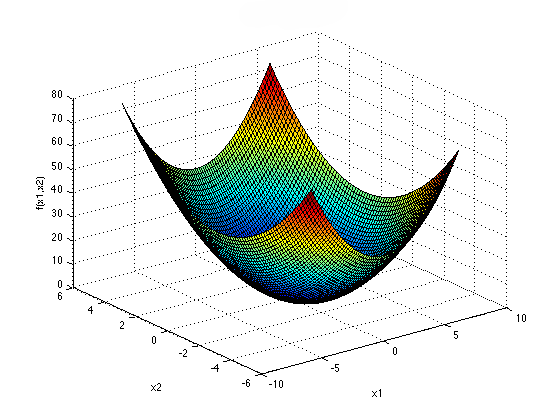
\includegraphics[width=\textwidth,height=\textheight,keepaspectratio]{sphere.png}
  \caption{Sphere's 2-dimensional graph function \cite{sf-uni-sp}}
\end{figure}

%%------------------------------------------------
 
\begin{table}[htbp]
\begin{minipage}{.4\linewidth}
    \centering

    \begin{tabular}{|c|c|c|c|c|}
    \hline
    D   & $\sigma$  & avg. time     & avg. sol.     & best sol. \\
    \hline
    10  & 0         & 89ms          & 0       & 0 \\
    \hline
    30  & 0         & 2.36s         & 0       & 0 \\
    \hline
    100 & 0         & 61.539s       & 0       & 0 \\
    \hline
    \end{tabular}
    \caption{Best improvement}
  \end{minipage}%
  \quad % ----------------------------------
  \begin{minipage}{.75\linewidth}
    \centering

    \begin{tabular}{|c|c|c|c|c|}
    \hline
    D   & $\sigma$  & avg. time     & avg. sol.     & best sol. \\
    \hline
    10  & 0         & 50ms          & 0             & 0 \\
    \hline
    30  & 0         & 1.21s         & 0             & 0 \\
    \hline
    100 & 0         & 32.58s        & 0             & 0 \\
    \hline
    \end{tabular}
    \caption{First improvement}
  \end{minipage}
\end{table}
\begin{table}[!htbp]
\begin{minipage}{.4\linewidth}
    \centering

    \begin{tabular}{|c|c|c|c|c|}
    \hline
    D   & $\sigma$  & avg. time     & avg. sol.     & best sol. \\
    \hline
    10  & 0         & 200ms         & 0             & 0 \\
    \hline
    30  & 0         & 4.98s         & 0             & 0 \\
    \hline
    \end{tabular}
    \caption{Worst improvement}
  \end{minipage}%
  \quad % ----------------------------------
  \begin{minipage}{.75\linewidth}
    \centering

    \begin{tabular}{|c|c|c|c|c|}
    \hline
    D   & $\sigma$  & avg. time     & avg. sol.     & best sol. \\
    \hline
    10  & 0         & 310ms         & 0             & 0 \\
    \hline
    30  & 0         & 4.97s         & 0             & 0 \\
    \hline
    100 & 0         & 152.95s       & 0             & 0 \\
    \hline
    \end{tabular}
    \caption{Simulated annealing}
  \end{minipage}
\end{table}

\newpage
\setcounter{table}{0}

%%------------------------------------------------

\subsection{Rastrigin}
$$ f(x) = A \cdot n + \sum_{i=1}^n \left[ x_i^2 - 10 \cdot cos(2 \pi x_i) \right] , x_i \in \left[ -5.12, 5.12 \right] $$

%%------------------------------------------------

\begin{figure}[!h]
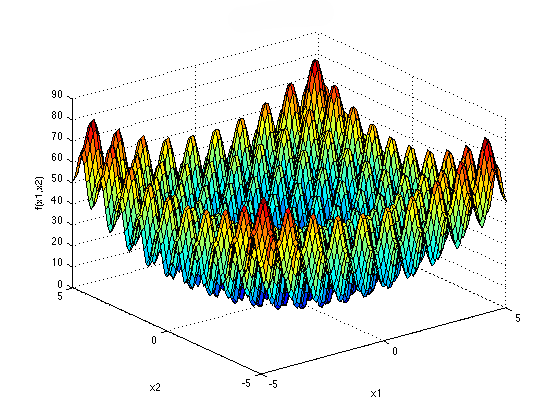
\includegraphics[width=\textwidth,height=\textheight,keepaspectratio]{rastrigin.png}
  \caption{Rastrigin's 2-dimensional graph function \cite{sf-uni-ra}}
\end{figure}

%%------------------------------------------------
    
\begin{table}[htbp]
\begin{minipage}{.4\linewidth}
    \centering
    
    \begin{tabular}{|c|c|c|c|c|}
    \hline
    D   & $\sigma$  & avg. time     & avg. sol.     & best sol.\\
    \hline
    10  & 0.53      & 307ms         & 1.96332       & 0.99496 \\
    \hline
    30  & 2.30      & 7.74s         & 22.49692      & 16.15900 \\
    \hline
    100 & 5.25      & 271.91s       & 124.04872     & 103.27991 \\
    \hline
    \end{tabular}
    \caption{Best improvement}
  \end{minipage}%
  \quad % ----------------------------------
  \begin{minipage}{.75\linewidth}
    \centering
    
    \begin{tabular}{|c|c|c|c|c|}
    \hline
    D   & $\sigma$  & avg. time     & avg. sol.     & best sol. \\
    \hline
    10  & 0.79      & 182ms         & 3.42327       & 1.23582 \\
    \hline
    30  & 2.63      & 4.37s         & 29.97694      & 22.84631 \\
    \hline
    100 & 4.99      & 154.12s       & 155.08213     & 141.60620 \\
    \hline
    \end{tabular}
    \caption{First improvement}
  \end{minipage}
\end{table}
\begin{table}[!htbp]
\begin{minipage}{.4\linewidth}
    \centering

    \begin{tabular}{|c|c|c|c|c|}
    \hline
    D   & $\sigma$  & avg. time     & avg. sol.     & best sol. \\
    \hline
    10  & 0.91      & 2.51s         & 5.12165       & 3.00004 \\
    \hline
    30  & 3.23      & 57.13s        & 38.18328      & 29.23457 \\
    \hline
    \end{tabular}
    \caption{Worst improvement}
  \end{minipage}%
  \quad % ----------------------------------
  \begin{minipage}{.75\linewidth}
    \centering

    \begin{tabular}{|c|c|c|c|c|}
    \hline
    D   & $\sigma$  & avg. time     & avg. sol.     & best sol. \\
    \hline
    10  & 0         & 19.81s        & 0       & 0 \\
    \hline
    30  & 0.86      & 171.31s       & 6.20453       & 3.99499 \\
    \hline
    100 & 1.94      & 19.16min      & 47.64466      & 40.26256 \\
    \hline
    \end{tabular}
    \caption{Simulated annealing}
  \end{minipage}
\end{table}

\newpage
\setcounter{table}{0}

%%------------------------------------------------

\subsection{Schwefel}
$$f(\mathbf{x}) = -\sum_{i=1}^{n} x_i \cdot \sin\left(\sqrt{|x_i|}\right) , x_i \in \left[-500,500\right]$$

%%------------------------------------------------

\begin{figure}[!h]
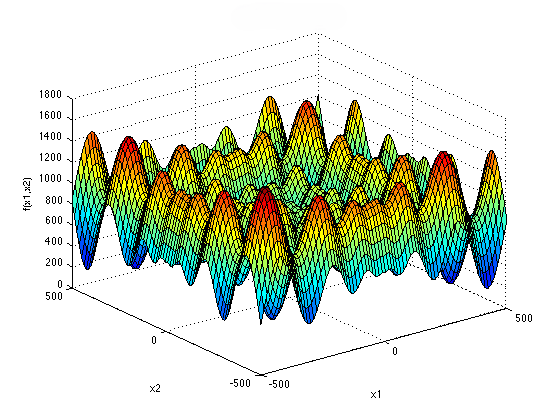
\includegraphics[width=\textwidth,height=\textheight,keepaspectratio]{schwefel.png}
  \caption{Schwefel's 2-dimensional graph function \cite{sf-uni-sw}}
\end{figure}
\vspace{0.5cm}

%%------------------------------------------------

\begin{table}[htbp]
\begin{minipage}{.4\linewidth}
    \centering

    \begin{tabular}{|c|c|c|c|c|}
    \hline
    D   & $\sigma$  & avg. time     & avg. sol.     & best sol. \\
    \hline
    10  & 18.4      & 755ms         & 17.70524      & 0.20936 \\
    \hline
    30  & 98.35     & 19.813s       & 894.62572     & 696.92139 \\
    \hline
    100 & 230.35    & 7,62min       & 5747.60089    & 5326.42004 \\
    \hline
    \end{tabular}
    \caption{Best improvement}
  \end{minipage}%
  \quad % ----------------------------------
  \begin{minipage}{.75\linewidth}
    \centering

    \begin{tabular}{|c|c|c|c|c|}
    \hline
    D   & $\sigma$  & avg. time     & avg. sol.     & best sol. \\
    \hline
    10  & 45.79     & 434ms         & 120.65099     & 34.54979 \\
    \hline
    30  & 111.23    & 11.18s        & 1464.46143    & 1186.97187 \\
    \hline
    100 & 217.08    & 261.82s       & 7615.11165    & 6976.11061 \\
    \hline
    \end{tabular}
    \caption{First improvement}
  \end{minipage}
\end{table}
\begin{table}[!htbp]
\begin{minipage}{.4\linewidth}
    \centering

    \begin{tabular}{|c|c|c|c|c|}
    \hline
    D   & $\sigma$  & avg. time     & avg. sol.     & best sol. \\
    \hline
    10  & 17.35     & 7.59s         & 212.34472     & 161.40279 \\
    \hline
    30  & 108.91    & 118.25s       & 1550.94308    & 1262.86526 \\
    \hline
    \end{tabular}
    \caption{Worst improvement}
  \end{minipage}%
  \quad % ----------------------------------
  \begin{minipage}{.75\linewidth}
    \centering

    \begin{tabular}{|c|c|c|c|c|}
    \hline
    D   & $\sigma$  & avg. time     & avg. sol.     & best sol. \\
    \hline
    10  & 0         & 22.98s        & 0.00037       & 0.00014 \\
    \hline
    30  & 0.07      & 173.01s       & 0.38921       & 0.21216 \\
    \hline
    100 & 41.02     & 25.93min      & 126.46816     & 71.91137 \\
    \hline
    \end{tabular}
    \caption{Simulated annealing}
  \end{minipage}
\end{table}

\newpage
\setcounter{table}{0}

%%------------------------------------------------

\subsection{Michalewicz}
$$f(\mathbf{x}) = -\sum_{i=1}^{n} \sin(x_i) \cdot \left(\sin\left(ix_i^2 / \pi\right)\right)^{2m} , m = 10, x_i \in \left[0,\pi\right]$$

%%------------------------------------------------

\begin{figure}[!h]
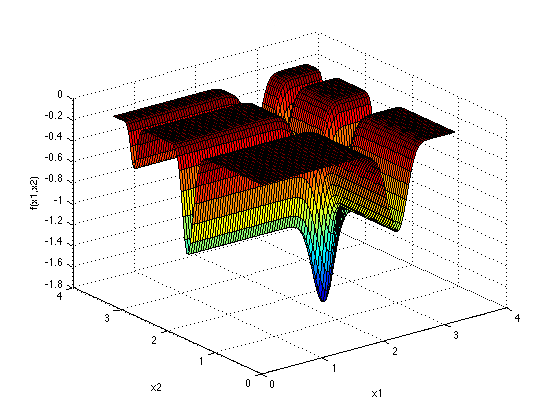
\includegraphics[width=\textwidth,height=\textheight,keepaspectratio]{michalewicz.png}
  \caption{Michalewicz's 2-dimensional graph function \cite{sf-uni-mc}}
\end{figure}
\vspace{0.5cm}

%%------------------------------------------------

\begin{table}[htbp]
\begin{minipage}{.4\linewidth}
    \centering

    \begin{tabular}{|c|c|c|c|c|}
    \hline
    D   & $\sigma$  & avg. time     & avg. sol.     & best sol. \\
    \hline
    10  & 0.04      & 1.50s         & -9.56506      & -9.65221 \\
    \hline
    30  & 0.28      & 33.42s        & -27.61249     & -28.56555 \\
    \hline
    100 & 0.51      & 9.73min       & -88.04727     & -89.11685 \\
    \hline
    \end{tabular}
    \caption{Best improvement}
  \end{minipage}%
  \quad % ----------------------------------
  \begin{minipage}{.75\linewidth}
    \centering

    \begin{tabular}{|c|c|c|c|c|}
    \hline
    D   & $\sigma$  & avg. time     & avg. sol.     & best sol. \\
    \hline
    10  & 0.05      & 865ms         & -9.50893      & -9.61160 \\
    \hline
    30  & 0.18      & 19.48s        & -27.02483     & -27.45056 \\
    \hline
    100 & 0.37      & 6.41min       & -73.07365     & -77.4654  \\
    \hline
    \end{tabular}
    \caption{First improvement}
  \end{minipage}
\end{table}
\begin{table}[!htbp]
\begin{minipage}{.4\linewidth}
    \centering

    \begin{tabular}{|c|c|c|c|c|}
    \hline
    D   & $\sigma$  & avg. time     & avg. sol.     & best sol. \\
    \hline
    10  & 0.12      & 7.39s         & -9.22340      & -9.42528 \\
    \hline
    30  & 0.29      & 104.44s       & -24.57051     & -25.19599 \\
    \hline
    \end{tabular}
    \caption{Worst improvement}
  \end{minipage}%
  \quad % ----------------------------------
  \begin{minipage}{.75\linewidth}
    \centering

    \begin{tabular}{|c|c|c|c|c|}
    \hline
    D   & $\sigma$  & avg. time     & avg. sol.     & best sol. \\
    \hline
    10  & 0         & 24.69s        & -9.65930      & -9.66015 \\
    \hline
    30  & 0.07      & 210.07s       & -29.11762     & -29.27980 \\
    \hline
    100 & 0.17      & 37.3min       & -95.99791     & -96.32860 \\
    \hline
    \end{tabular}
    \caption{Simulated annealing}
  \end{minipage}
\end{table}

%%------------------------------------------------

\subsection{Interpretation}

\subparagraph{}
The experimental results demonstrate that \textit{\textbf{Best Improvement}} consistently outperforms \textit{\textbf{First Improvement}} in solution quality across all test functions, particularly in higher dimensions, however at a higher computational cost. \textit{\textbf{Simulated annealing}} exhibits superior performance by escaping local optima, especially notable for \textbf{Rastrigin} and \textbf{Schwefel} functions, yielding better outputs when compared against \textit{\textbf{Best Improvement}}. Finally, \textit{\textbf{Worst Improvement}} showed inferior results at a higher computational cost than all other strategies.

\section{Conclusions}

\subparagraph{}
Looking into our results, it can safely be stated that the Hill Climbing algorithm is efficient and succeeds in delivering significant values, in the search for the global minimum. Comparing it with the deterministic approach, the time is much less than the brute-force traversal of the graph function. The different improvement settings showcase diverse trade-offs between these designs which can be further exploited. \\

An exemplary observation would be the Simulated annealing contributions; they usually bring better solutions that are scalable for real competitive environments. It's useful in concrete cases, even though considerable time intervals were detected. \\

Overall, this study provides valuable insights into the application of optimization algorithms in solving complex optimization problems and contributes to the understanding of their performance across different dimensions. 

%%------------------------------------------------
%% bibliography

\begin{thebibliography}{9}

\bibitem{m}
    Metropolis \url{https://www.sciencedirect.com/topics/computer-science/metropolis-algorithm} \\  
  
\bibitem{course}
  Course page \\ Hill Climbing documentation.
  \url{https://profs.info.uaic.ro/eugen.croitoru/teaching/ga/}

\bibitem{cuda}
  Nvidia Cuda coalesced memory \\
  \url{https://docs.nvidia.com/cuda/cuda-c-best-practices-guide/index.html\# coalesced-access-to-global-memory}

\bibitem{sf-uni-sp}
  Simon Fraser University \\ Sphere's function.
  \url{https://www.sfu.ca/~ssurjano/spheref.html}

\bibitem{sf-uni-ra}
  Simon Fraser University \\  Rastrigin's function.
  \url{https://www.sfu.ca/~ssurjano/rastr.html}

\bibitem{sf-uni-sw}
  Simon Fraser University \\ Schwefel's function.
  \url{https://www.sfu.ca/~ssurjano/schwef.html}

\bibitem{sf-uni-mc}
  Simon Fraser University \\ Michalewicz's function.
  \url{https://www.sfu.ca/~ssurjano/michal.html}

\bibitem{l}
  Overleaf \\ LaTeX training.
  \url{https://tex.stackexchange.com/questions/39017/how-to-influence-the-position-of-float-environments-like-figure-and-table-in-lat/39020#39020} \\
  \url{https://latex-cookbook.net/function-plot/%7D} \\  
  \url{https://www.overleaf.com/learn/latex/Learn_LaTeX_in_30_minutes%7D}

\end{thebibliography}  
\end{document}
